% Offizielle Beispieldatei für beamer-Vorlage aus tubslatex Version 0.3beta2
\documentclass[fleqn,11pt,aspectratio=43]{beamer}

\usepackage[english]{babel}
\usepackage[utf8x]{inputenc}
\usepackage{graphicx}
\usepackage{bm} 
\usepackage{amsmath}
\usepackage{xcolor}
\usepackage{subcaption}
\usepackage[font={footnotesize,it},skip=2pt]{caption}
\definecolor{DGTU}{HTML}{760054}

\usepackage{bbm} %for probability notation#


\usetheme[%
  nexus,%        Nexus Fonts benutzen
  lnum,%         Versalziffern verwenden
  %cmyk,%<rgbprint>,          Auswahl des Farbmodells
  green,%<blue/orange/green/violet> Auswahl des Sekundärfarbklangs
  medium,%<dark,light,medium>        Auswahl der Helligkeit
  colorhead,%    Farbig hinterlegte Kopfleiste
  colorfoot,%    Farbig hinterlegt Fußleiste auf Titelseite
  colorblocks,%   Blöcke Farbig hinterlegen
  %nopagenum,%    Keine Seitennumer in Fußzeile
  %nodate,%       Kein Datum in Fußleiste
  tocinheader,%   Inhaltsverzeichnis in Kopfleiste
  %tinytocinheader,% kleines Kopfleisten-Inhaltsverzeichnis
  %widetoc,%      breites Kopfleisten-Inhaltsverzeichnis
  %narrowtoc,%    schmales Kopfleisten-Inhaltsverzeichnis
  %nosubsectionsinheader,%  Keine subsections im Kopfleisten-Inhaltsverzeichnis
  %nologoinfoot,% Kein Logo im Fußbereich darstellen
  ]{tubs}

% Titelseite
\title{A Statistical Approach for the Fusion of
Data and Finite Element Analysis in
Vibroacoustics}
\subtitle{Defense of the Master's Thesis\\ Supervision: Prof. Langer, Prof. Römer, M.Sc. Sreekumar}
\author{Lucas Hermann}
% Titelgrafik, automatisch beschnitten, Weitere Optionen: <scaled/cropx/cropy>
%\titlegraphic[cropped]{\includegraphics{titlepicture.png}}
\titlegraphic[scaled]{\includegraphics{titlepicture.png}}

% Logo, dass auf Titelseiten oben rechts und auf Inthaltsseiten unten rechts
% dargestellt wird. Es wird jeweils automatisch skliert
\logo{\includegraphics{InA-Logo-rgb.pdf}}
%\logo{Institut für Unkreativität\\und Schreibschwäche}

\begin{document}

\begin{frame}[plain]
\titlepage
\end{frame}
\begin{frame}{Content}
%\tableofcontents[part=1]
%
%\tableofcontents[part=2]
%
%\tableofcontents[part=3]
\begin{itemize}
\item Objectives
\item Prerequisites
\item statFEM
\item 1D example
\item 2D Helmholtz example
\item Conclusion and Outlook

\end{itemize}
\end{frame}
\part{Objectives}

\begin{frame}[plain]
  \partpage
\end{frame}


\section{Objectives}





\begin{frame}{Objectives}
The goals of the thesis are:
\begin{itemize}
	\item to understand and explain statFEM (statistical FEM) using a practical example
 	\item to implement a statFEM approach for vibroacoustics using the Helmholtz equation
  \item to provide a means to use sparse sensor data to improve the accuracy of an FEM solution and to quantify uncertainty
  \item to gain insight on the limits and possibilities of statFEM in vibroacoustics
  %\item to present a possible use case of the method
  %\item to use a non-parametric approach to increase the accuracy of the solution without touching the FEM itself
\end{itemize}

\end{frame}



\begin{frame}{Objectives}
Hypotheses: \\

\begin{itemize}
	\item uncertainty in parameters of the PDE will lead to uncertainty in the solution
	\item introducing observation data will decrease the overall variance
	\item the more data is introduced, the less probability mass will be on the FEM solution prior
\end{itemize}



\end{frame}



\begin{frame}{Objectives}

Motivation:
\begin{itemize}
  \item Merge FEM and data while quantifying uncertainty:
   Apply statFEM to an FEM solution to reduce the model error
      
 
 % \begin{itemize}
  %  \item Unterpunkte ebenfalls
   % \item Allerdings etwas kleiner
  %\end{itemize}
\end{itemize}

\begin{figure}[h]
\begin{center}
\includegraphics[scale=1]{intro}
\end{center}
\end{figure}

\end{frame}










\part{Prerequisites}
\begin{frame}[plain]
  \partpage
\end{frame}





\section{Prerequisites}


\subsection{Modeling data}
\begin{frame}{Prerequisites: Data}

\begin{block}{Statistical Model}
The vector of measured data $\bm{y}$ can be described as a combination of different parts:
\begin{equation*}
\bm{y} = \textcolor{DGTU}{\bm{z}} + \textcolor{olive}{\bm{e}} = \textcolor{DGTU}{\rho \bm{P} \bm{u} + \bm{d}} + \textcolor{olive}{\bm{e}}
\end{equation*}
\end{block}
$\textcolor{DGTU}{\bm{z}}$: The true solution\\
$\textcolor{olive}{\bm{e}}$: Measurement error\\
$\bm{u}$: Original FEM solution\\
$\rho \bm{P} \bm{u}$: Scaled projected FEM solution ($\bm{P}$ is the projection matrix)\\

$\bm{d} \sim \mathcal{GP}(\bar{\bm{d}}, \bm{C}_d)$: Model mismatch
\end{frame}


\subsection{Gaussian Processes}
\begin{frame}{Prerequisites: Gaussian Processes}
\begin{block}{Gaussian Processes:}
A GP $\bm{u} \sim \mathcal{GP}(\bar{\bm{u}},\bm{C}_u)$ is a distribution of functions. It is defined by a mean $\bar{\bm{u}}$ and a covariance matrix $\bm{C}_u$. It is the limit of a multivariate Gaussian distribution (i.e. one with infinitely many dimensions).

\end{block}
      	\begin{figure}[h]
		\begin{center}
		\includegraphics[width=.9\textwidth]{GPExpl.pdf}
		\end{center}
		\caption{Conditioning a GP on data (black dots) yields a new GP with decreased variance around the sensor positions.}
		\end{figure}

\end{frame}

%\begin{frame}{Prerequisites: Gaussian Processes}
%\begin{figure}[!ht]
%\begin{center}
%\includegraphics[width=0.7\textwidth]{bivarGP}
%\caption{Visual explanation of the intuition behind GPs}
%\label{fig:bivarGP}
%\end{center}
%\end{figure}
%\end{frame}


%
%\begin{frame}{Prerequisites: Gaussian Processes}
%\begin{figure}[!ht]
%\begin{center}
%\includegraphics[width=0.9\textwidth]{multivarGP}
%\caption{Visual explanation of the intuition behind GPs}
%\label{fig:multiGP}
%\end{center}
%\end{figure}
%\end{frame}





%\begin{frame}{Prerequisites: Gaussian Processes}
%\begin{block}{Squared Exponential Kernel:}
%A kernel is a \emph{covariance function}.  It continuously describes the covariance between different points in the calculation domain and describes the expected behaviour of the approximated function.
%\begin{equation}
%k_{SE} = \sigma \exp \left( -\frac{||x-x'||^2}{2l^2} \right)
%\end{equation}
%\end{block}
%$\sigma$: standard deviation\\
%$l$: distance measure\\
%Evaluating the kernel at a defined set of points (e.g. nodes in an FEM mesh) yields the covariance matrix.
%\end{frame}


\begin{frame}{Prerequisites: Gaussian Processes}
A kernel is a \emph{covariance function}.  It continuously describes the covariance between different points in the calculation domain and describes the expected behaviour of the approximated function.
\begin{block}{Mat\'ern Kernel:}
\begin{equation*}
k_M(r) = \sigma^2 \frac{2^{1-\nu}}{\Gamma(\nu)}  \left( \frac{\sqrt{2\nu}r}{l}  \right)^{\nu} K_{\nu}  \left(  \frac{\sqrt{2\nu}r}{l}   \right)
\label{eqn:MaternKernel}
\end{equation*}
\end{block}
$\sigma$: standard deviation\\
$l$: correlation length\\
$\nu$: free parameter\\

Choosing a kernel means giving prior information on the expected shape of the resulting functions.%
%The higher $\nu$, the closer the kernel comes to the squared exponential kernel.
%Evaluating the kernel at a defined set of points (e.g. nodes in an FEM mesh) yields the covariance matrix.
\end{frame}


%\begin{frame}{Prerequisites: Gaussian Processes}
%      	\begin{figure}[h]
%		\begin{center}
%		\includegraphics[width=1\textwidth]{GPExpl.pdf}
%		\end{center}
%		\caption{Conditioning a GP on data (black dots) yields a new GP with decreased variance around the sensor positions.}
%		\end{figure}
%\end{frame}



\subsection{Bayesian Inference}
\begin{frame}{Prerequisites: Bayesian Inference}
\begin{block}{Bayes' law:}
Conditioning a distribution $\bm{u}$ on data $\bm{y}$ requires a prior for the distribution $p(\bm{u})$ and a likelihood for the data $p(\bm{y}|\bm{u})$.
\begin{equation*}
p(\bm{u}|\bm{y}) = \frac{p(\bm{y}|\bm{u})p(\bm{u})}{p(\bm{y})}
\end{equation*}
\end{block}
The prior is the stochastic FEM solution.\\
The likelihood can be derived from the statistical model ($\bm{y} = \textcolor{DGTU}{\rho \bm{P} \bm{u} + \bm{d}} + \textcolor{olive}{\bm{e}}$) in which all components are Gaussian.\\
The marginal likelihood $p(\bm{y})$ is the probability for the data averaged over all possible prior solutions.
\end{frame}











\part{The statFEM procedure}
\begin{frame}[plain]
  \partpage
\end{frame}


\section{statFEM}





\begin{frame}{statFEM: Bayesian Inference}
Assuming the stochastic FEM solution to be a GP, the posterior GP can be infered using the statistical model for the data.
\begin{block}{Inference of the posterior GP:}
The posterior solution is going to be a GP: \\
$\bm{u}_{|y} \sim \mathcal{GP}(\bar{\bm{u}}_{|y}, \bm{C}_{u|y})$.
\begin{equation*}
\bm{\bar{u}}_{|y} = \bm{C}_{\bm{u}|\bm{y}} \left(   \rho \bm{P}^T  (\bm{C}_d + \bm{C}_e)^{-1}  \bm{y}  +  \bm{C}_u^{-1}  \bar{\bm{u}}   \right)
\end{equation*}
\begin{equation*}
\bm{C}_{\bm{u}|\bm{y}} = \left(      \rho^2  \bm{P}^T   (\bm{C}_d + \bm{C}_e)^{-1}  \bm{P}  +  \bm{C}_u^{-1}    \right)^{-1} 
\end{equation*}
\end{block}
Using an optimization method, the hyperparameters for $\bm{C}_d$ are determined.

\end{frame}











%\section{Estimation of Hyperparameters}
\begin{frame}{statFEM: Estimation of Hyperparameters}
Bayes' rule for the hyperparameters:
\begin{equation*}
p(\bm{w}|\bm{y}) = \frac{p(\bm{y}|\bm{w}) p(\bm{w})}{\int p(\bm{y}|\bm{w}) p(\bm{w}) \, \mathrm{d}\bm{w}}
\label{eqn:bayesHyperp}
\end{equation*}
with $\bm{w}$ the vector of hyperparameters and $\bm{y}$ the observations vector.
For an uninformative prior there holds $p(\bm{w}|\bm{y}) \propto p(\bm{y}|\bm{w})$ and it can be shown that ($\bm{K}$ is a covariance matrix, $n$ the number of observations)
\begin{block}{negative log likelihood:}
\begin{equation*}
- \log p(\bm{y}|\bm{w}) = \frac{n}{2} \log(2 \pi) + \frac{1}{2} \log |\bm{K}| + \frac{1}{2}(\rho \bm{P}\bar{\bm{u}} - \bm{y})^T \bm{K}^{-1} (\rho \bm{P}\bar{\bm{u}} - \bm{y}) \;,
\label{eqn:neglog}
\end{equation*}
which is minimized (with e.g. MCMC or L-BFGS) to find the optimal set of hyperparameters.
\end{block}
 
\end{frame}


\section{1D example}
\subsection{Setting}

\begin{frame}{Setting: 1D Poisson}
To test the methods and code, the well-known Poisson example was solved in 1D.
\begin{block}{Weak form:}
The uncertainty is in the source term: $\bm{f} \sim \mathcal{GP}(\bar{\bm{f}}, \bm{C}_f)$
\begin{equation*}
-\int_{\Omega} \nabla p \cdot \nabla v \,\mathrm{d}x = \int_{\Omega} \bm{f}v \,\mathrm{d}x
\end{equation*}
\end{block}
      	\begin{figure}[h]
		\begin{center}
		\includegraphics[width=0.6\textwidth]{1dDomain}
		\end{center}
		\end{figure}

\end{frame}


\subsection{FEM solution}
\begin{frame}{FEM solution: 1D Poisson}
The FEM solution serves as a prior and is modeled as a GP with a mean and variance. Arbitrarily many samples can be drawn from it. A GP for the 'true' solution (here $z$) is created.
      	\begin{figure}[h]
		\begin{center}
		\includegraphics[width=0.75\textwidth]{FEMprior_Z}
		\end{center}
		\end{figure}

\end{frame}


\subsection{Inference}
\begin{frame}{Infered solution: 1D Poisson}
1 sensor, 1 observation
      	\begin{figure}[h]
		\begin{center}
		\includegraphics[width=0.7\textwidth]{1DPost_1P1O}
		\end{center}
		\end{figure}

	\end{frame}


\begin{frame}{Infered solution: 1D Poisson}
4 sensors, 1 observation each
      	\begin{figure}[h]
		\begin{center}
		\includegraphics[width=0.7\textwidth]{1DPost_4P1O}
		\end{center}
		\end{figure}

	\end{frame}

\begin{frame}{Infered solution: 1D Poisson}
4 sensors, 20 observations each
      	\begin{figure}[h]
		\begin{center}
		\includegraphics[width=0.7\textwidth]{1DPost_4P20O}
		\end{center}
		\end{figure}

	\end{frame}

%\begin{frame}{Infered solution: 1D Poisson}
%Only partial data available: FEM prior still determines overall shape
%\begin{figure}[!ht]
%
%	\begin{subfigure}[t]{.5\textwidth}
%	\centering
%	\includegraphics[width=1\linewidth]{Results/1D/HalfSide/Model_Error/5o_15s/Result.pdf}
%	\caption{With model error. $n_p=15$, $n_o=5$}
%		\label{fig:1DOneSideda}
%	\end{subfigure}%
%	\begin{subfigure}[t]{.5\textwidth}
%	\centering
%	\includegraphics[width=1\linewidth]{Results/1D/HalfSide/Model_Error/100o_15s/Result.pdf}
%	\centering
%	\caption{With model error. ${n_p=15}$, ${n_o=100}$ }
%	\label{fig:1DOneSidedb}
%	\end{subfigure}
%	
%
%\caption{Posterior of the 1D example for observations only on one side of the domain}
%\label{fig:1DOneSided}
%\end{figure}
%
%	\end{frame}
	

%\begin{frame}{Infered solution: 1D Poisson}
%Only partial data available: FEM prior still determines overall shape
%\begin{figure}[!ht]
%
%	
%	
%	\begin{subfigure}[t]{.5\textwidth}
%	\centering
%	\includegraphics[width=1\linewidth]{Results/1D/HalfSide/No_Model_Error/5o_15s/Result.pdf}
%	\caption{Without model error, only 0.75x\\
%	 scaling. ${n_p=15}$, ${n_o=5}$}
%		\label{fig:1DOneSidedc}
%	\end{subfigure}%
%	\begin{subfigure}[t]{.5\textwidth}
%	\centering
%	\includegraphics[width=1\linewidth]{Results/1D/HalfSide/No_Model_Error/100o_15s/Result.pdf}
%	%\centering
%	\caption{Without model error, only 0.75x scaling. ${n_p=15}$, ${n_o=100}$}
%	\label{fig:1DOneSidedd}
%	\end{subfigure}
%
%\caption{Posterior of the 1D example for observations only on one side of the domain}
%\label{fig:1DOneSided}
%\end{figure}
%
%	\end{frame}
	
	
	
	
\begin{frame}{Infered solution: 1D Poisson}
Prior-data conflict: The further away from the prior mean data is observed, the more observations are needed to match the mean.
\begin{figure}[!ht]
\centering
	\begin{subfigure}[t]{.5\textwidth}
	\centering
	\includegraphics[width=1\linewidth]{../../Python/Results/1D/PriorDataConflict/Model_Error/30s_5o/Result.pdf}
	\caption{With model error. $n_p=30$, $n_o=5$}
		\label{fig:1DConflicta}
	\end{subfigure}%
	\begin{subfigure}[t]{.5\textwidth}
	\centering
	\includegraphics[width=1\linewidth]{../../Python/Results/1D/PriorDataConflict/Model_Error/30s_100o/Result.pdf}
\centering
\caption{With model error. $n_p=30$, $n_o=100$ }
\label{fig:1DConflictb}
	\end{subfigure}
	
\caption{Posterior of the 1D example for observations far outside the FEM prior variance band}
\label{fig:1DConflict}
\end{figure}

	\end{frame}	
	
	
	
	
	

	

	
\section{2D Helmholtz}
\subsection{Setting}

\begin{frame}{Setting: 2D Helmholtz}
\begin{block}{Weak form:}
The \textcolor{DGTU}{uncertainty} is in the boundary term.
\begin{equation*}
-\int_{\Omega} \nabla p \cdot \nabla v \,\mathrm{d}\Omega + \textcolor{DGTU}{\oint_{\Gamma} v \nabla p  \,\mathrm{d}\Gamma}+ \int_{\Omega} k^2 pv \,\mathrm{d}\Omega = 0
\label{eqn:WeakHelmholtz}
\end{equation*}
\end{block}

\begin{columns}[onlytextwidth]
    \column{0.5\textwidth}
    \begin{block}{Neumann boundary:}
      $\oint_{\Gamma_N} v (\rho \omega^2 \textcolor{DGTU}{\vec{D}}\vec{n})  \,\mathrm{d}\Gamma$\\
      $\textcolor{DGTU}{\vec{D}}$: Piston displacement
          \end{block}
          1D boundary function $\textcolor{DGTU}{D(y)}$: $\textcolor{DGTU}{D \sim \mathcal{GP}(\bar{\bm{g}}, \bm{C}_g)}$
  %    For $\vec{U} = 0$: Natural (reflecting) BC on $\Gamma_{N0}$
    \column{0.5\textwidth}
      	\begin{figure}[h]
		\begin{center}
		\includegraphics[width=0.75\textwidth]{BCsThesis1}
		\end{center}
		\end{figure}
  \end{columns}
\end{frame}


\subsection{FEM solution}
\begin{frame}{FEM solution: 2D Helmholtz}
The FEM solution serves as a prior and is modeled as a GP with a mean and variance. Arbitrarily many samples can be drawn from it. 
      	\begin{figure}
      	\begin{columns}
      	
      	\column{.65\linewidth}
		\includegraphics[width=1\textwidth]{SolutionCustom2D.pdf}
		\column{.2\linewidth}
		\caption{Overview of the source and prior GP}
		\end{columns}


		\end{figure}


\end{frame}





\subsection{Inference}

\begin{frame}{Inferred solution: 2D Helmholtz, Variance fields}

Variance drops with increasing number of sensors and/or number of observations.
\begin{figure}
\begin{columns}
\column{.7\linewidth}
\includegraphics[width=1\textwidth]{../../Python/Results/2D/100procent_no_d/VarField_Posterior.pdf}
\column{.2\linewidth}
\caption{Posterior of the 2D Helmholtz equation example for different numbers of sensors and observations}
\end{columns}
\end{figure}


\end{frame}



%\begin{frame}{Inferred solution: 2D Helmholtz}
%Observations on a scaled sample of a realization of the FEM prior lead to a correctly scaled posterior. The model error is close to zero.
%\begin{figure}[!ht]
%	\begin{columns}
%      	
%      	\column{.7\linewidth}
%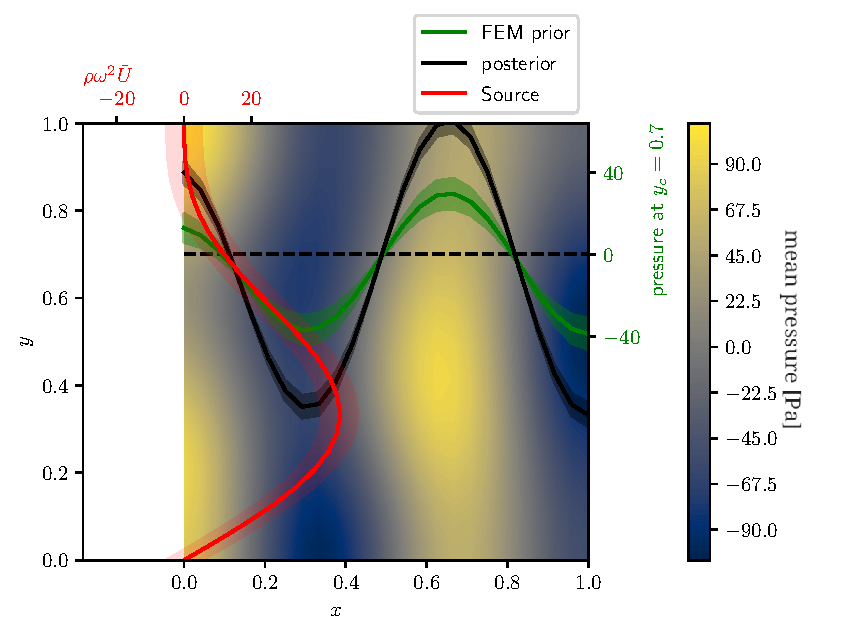
\includegraphics[width=1\textwidth]{../../Python/Results/2D/75procent_no_d/SolutionCustomPosterior.pdf}
%\centering
%\column{.2\linewidth}
%\caption{Source, prior and posterior for the 2D example at 500Hz. Observations taken on 0.75x scaling of a realization of the FEM prior.}
%\end{columns}
%\end{figure}
%
%	\end{frame}
%





\begin{frame}{Inferred solution: observations with error}
When observing on a GP which is not a realization of the prior GP, statFEM can create a new GP which fits the data. The model error is greater than zero.
\begin{figure}[!ht]
\includegraphics[width=0.8\textwidth]{3dTest.pdf}
\centering
\caption{Comparison of prior and posterior in a 3D view for the observations with model error. Mean Squared Error (MSE) for comparison.}
\end{figure}
\end{frame}


\begin{frame}{Inferred solution: prior-data conflict}
If data is observed far outside the confidence intervals of the prior, the procedure is not able to match the posterior perfectly to the data. More sensor locations and observations are necessary.
\begin{figure}
\includegraphics[width=.8\textwidth]{../../Python/Results/2D/prior_data_conflict/3dMSE.pdf}
\centering
\caption{Comparison of prior and posterior for the observations with a prior-data conflict}
\end{figure}

\end{frame}



\begin{frame}{Inferred solution: constrained measurement domain}
For observations only in a part of the domain, the variance becomes lower in the whole domain but especially in regions where sensors are placed.
\begin{figure}[!ht]
\includegraphics[width=0.8\textwidth]{../../Python/Results/2D/HalfSide/3/HalfSide.pdf}
\centering
\caption{Prior and posterior variance compared for 500Hz and sensor locations only in the upper half of the domain. }
\label{fig:VarianceHalfSided2D}
\end{figure}
\end{frame}




\begin{frame}{Inferred solution: constrained measurement domain}
The variance can still be lowered throughout the domain by increasing the number of sensors and observations.
\begin{figure}
\begin{columns}
\column{.7\linewidth}
\includegraphics[width=1\textwidth]{../../Python/Results/2D/HalfSide/4/VarField_Posterior.pdf}
\column{.2\linewidth}
\caption{Posterior variance for $500 \,\mathrm{Hz}$ and sensor locations only in the upper half of the domain. }
\end{columns}
\end{figure}

\end{frame}



\part{Outlook}

\begin{frame}[plain]
  \partpage
\end{frame}

\section{Conclusion}
\begin{frame}{Conclusion}
\begin{itemize}
\item a working statFEM approach for vibroacoustics was developed
\item small variances in the Neumann BC lead to strong variances in the solution
\item by introducing observations, the variance can be lowered drastically
\item the FEM prior is properly scaled to given data\\

\item limits of the method lie in poorly scaled FEM priors and sparse available data
\end{itemize}
\end{frame}

\section{Outlook}
\begin{frame}{Outlook}
Only very few possibilities have been show here. It is important to find out more about:
\begin{itemize}
\item uncertainties in different classes of boundaries such as impedance boundary conditions and in material parameters
\item different choices of kernels for the boundary function
\item kernels with frequency dependence
\item convergence behavior of the method
\item sensor placement algorithm
\end{itemize}
\end{frame}


\part{Endpage}

\begin{frame}[plain]
  Thank you for your attention and feel free to ask questions!\\
  
  \begin{figure}

\includegraphics[width=0.7\textwidth]{refs.png}

\end{figure}

\end{frame}



\end{document}










